\section{Chương 1: Tóm tắt và phân tích bài báo DINOv2}

\subsection{Bài toán (Problem)}
Trong lĩnh vực Thị giác máy tính (Computer Vision), việc học các đặc trưng hình ảnh (visual features) mạnh mẽ thường phụ thuộc nặng nề vào các tập dữ liệu khổng lồ được gán nhãn thủ công (ví dụ: ImageNet). Tuy nhiên, phương pháp Học có giám sát (Supervised Learning) này bộc lộ hai điểm yếu chí mạng: (1) Chi phí và thời gian gán nhãn vô cùng đắt đỏ; (2) Giới hạn về khả năng bao phủ sự đa dạng của thế giới thực (vấn đề phân phối đuôi dài - long-tail distribution).

Để giải quyết vấn đề này, các mô hình học từ cặp dữ liệu văn bản - hình ảnh (như CLIP hay OpenCLIP) đã ra đời và đạt được thành công lớn. Dù vậy, các mô hình này lại gặp phải rào cản về "nút thắt ngôn ngữ" (text bottleneck): Văn bản chỉ mô tả được ý nghĩa toàn cục (global semantics) của bức ảnh, nhưng hoàn toàn bất lực trong việc mô tả chi tiết các thông tin về hình học, không gian, hay ranh giới vật thể ở cấp độ pixel.

Do đó, bài toán cốt lõi mà DINOv2 đặt ra là: Làm thế nào để xây dựng một mô hình nền tảng thuần túy cho thị giác máy tính, có khả năng tự động học từ hình ảnh không nhãn (Self-Supervised Learning - SSL), nhưng xuất ra được các "đặc trưng vạn năng" (all-purpose features)? Các đặc trưng này phải hoạt động xuất sắc ở cả cấp độ toàn cục (hiểu ngữ nghĩa bức ảnh) lẫn cấp độ cục bộ (chi tiết từng pixel cho các tác vụ không gian/hình học).

\subsection{Động lực nghiên cứu (Motivation)}
Động lực của nhóm nghiên cứu tại Meta AI xuất phát từ sự thành công vang cụ của các Mô hình Ngôn ngữ lớn (LLMs) trong lĩnh vực Xử lý Ngôn ngữ Tự nhiên (NLP). Các LLM có thể học từ lượng dữ liệu văn bản thô khổng lồ trên Internet nhờ một nhiệm vụ tự giám sát tự nhiên (dự đoán từ tiếp theo).

Tuy nhiên, trong Thị giác máy tính, việc sao chép quy mô này gặp khó khăn nghiêm trọng. Dữ liệu hình ảnh trên Internet không có cấu trúc, chứa đầy nhiễu và rất thiếu cân bằng. Nếu đưa trực tiếp hàng tỷ bức ảnh thô này vào huấn luyện, mô hình sẽ không hội tụ hoặc học phải những đặc trưng vô giá trị.

Từ đó, động lực chính của DINOv2 được xác định qua hai hướng tiếp cận đột phá:
\begin{itemize}
    \item \textbf{Về dữ liệu:} Thay vì sử dụng dữ liệu không chọn lọc (uncurated data), cần phải có một hệ thống tự động để tinh lọc ra một tập dữ liệu "vàng" khổng lồ, đa dạng nhưng vẫn giữ được chất lượng tương đương dữ liệu có nhãn thủ công.
    \item \textbf{Về thuật toán:} Cần xây dựng một cơ chế học tự giám sát ổn định để huấn luyện các mạng Vision Transformer (ViT) ở quy mô hàng tỷ tham số (1B parameters) mà không bị "sụp đổ đặc trưng" (representation collapse - hiện tượng mô hình dự đoán ra cùng một đầu ra cho mọi đầu vào).
\end{itemize}

\subsection{Phương pháp đề xuất (Method)}
DINOv2 không đơn thuần là một thuật toán mới, mà là một hệ thống (pipeline) hoàn chỉnh kết hợp giữa kỹ nghệ dữ liệu và tối ưu hóa huấn luyện. Phương pháp được chia thành các trụ cột chính:

\textbf{a. Quy trình Giám tuyển Dữ liệu (Data Curation Pipeline):} \\
Nhóm tác giả không gán nhãn thủ công mà tự động hóa việc xây dựng tập dữ liệu thông qua cơ chế Truy xuất hình ảnh (Image Retrieval). Cụ thể:
\begin{itemize}
    \item Họ sử dụng một tập dữ liệu nhỏ đã được giám tuyển chất lượng cao (Curated data) làm "hạt giống".
    \item Trích xuất đặc trưng của tập hạt giống này và so sánh độ tương đồng cosine (Cosine similarity) với hàng tỷ bức ảnh thô cào được từ web.
    \item Chỉ những bức ảnh từ web có độ tương đồng cao với tập hạt giống mới được giữ lại. Kết quả là sự ra đời của LVD-142M – tập dữ liệu gồm 142 triệu hình ảnh chất lượng cao, cân bằng về mặt phân phối mà không cần bất kỳ sự can thiệp nào của con người.
\end{itemize}

% \begin{figure}[h]
%     \centering
%     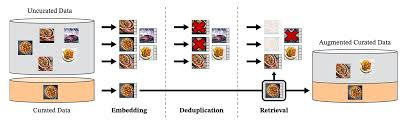
\includegraphics[width=0.9\textwidth]{figures/download.jpeg}
%     \caption{Quy trình xây dựng tập dữ liệu (Data Curation Pipeline) của DINOv2}
%     \label{fig:data_curation}
% \end{figure}

\textbf{b. Mục tiêu Huấn luyện Kép (Dual Training Objective):} \\
Thuật toán của DINOv2 là sự hợp nhất của hai phương pháp SSL tiên tiến, học theo kiến trúc Student-Teacher:
\begin{itemize}
    \item \textbf{Học đặc trưng toàn cục (DINO - Self-Distillation):} Mạng Student học cách dự đoán lại biểu diễn toàn cục (global embedding) của mạng Teacher. Trọng số của Teacher được cập nhật từ từ thông qua Trung bình động theo cấp số nhân (EMA - Exponential Moving Average) từ trọng số của Student.
    \item \textbf{Học đặc trưng cục bộ (iBOT - Masked Image Modeling):} Tương tự như trò chơi điền vào chỗ trống, mô hình sẽ bị che đi (mask) một số mảnh ảnh (patches). Mạng Student buộc phải khôi phục lại các đặc trưng của những mảnh bị che này dựa trên thông tin từ các mảnh lân cận. Điều này ép mô hình phải hiểu sâu về cấu trúc không gian.
\end{itemize}

\textbf{c. Các kỹ thuật ổn định mô hình (Regularization \& Engineering):} \\
Để huấn luyện thành công mạng ViT-g (1 tỷ tham số), nhóm nghiên cứu áp dụng các công cụ toán học tối tân để tránh mô hình bị sụp đổ:
\begin{itemize}
    \item \textbf{Sử dụng Sinkhorn-Knopp Centering:} Tối ưu hóa việc phân cụm các đặc trưng.
    \item \textbf{Sử dụng KoLeo Regularizer:} Hàm phạt giúp các vector đặc trưng phân bố đều đặn và cách xa nhau trong không gian biểu diễn (representation space).
    \item \textbf{Tăng độ phân giải ở giai đoạn cuối (High-resolution fine-tuning):} Ở những epoch cuối, mô hình được huấn luyện với ảnh đầu vào có độ phân giải cao hơn để làm mịn các đặc trưng ở cấp độ pixel.
\end{itemize}

\subsection{Kết quả đạt được (Result)}
DINOv2 đã tạo ra một cơn địa chấn trong cộng đồng nghiên cứu khi chứng minh rằng các đặc trưng học tự giám sát thuần túy có thể đánh bại các mô hình có giám sát truyền thống.
\begin{itemize}
    \item \textbf{Đặc trưng "Out-of-the-box" mạnh mẽ:} Không cần phải tinh chỉnh lại toàn bộ mạng (fine-tuning) cho từng bài toán mới. Chỉ cần đóng băng (freeze) bộ trọng số của DINOv2 và thêm một lớp phân loại tuyến tính đơn giản (Linear Probing) hoặc dùng thuật toán k-NN, mô hình đã đạt kết quả SOTA (State-of-the-Art) trên tập ImageNet-1K.
    \item \textbf{Thống trị các tác vụ dự đoán dày đặc (Dense Tasks):} Đây là điểm vượt trội nhất của DINOv2 so với mô hình CLIP. DINOv2 cho ra kết quả cực kỳ chính xác trong các bài toán yêu cầu hiểu chi tiết hình học như: Phân đoạn ngữ nghĩa (Semantic Segmentation) và Ước lượng chiều sâu đơn mục kính (Monocular Depth Estimation).
    \item \textbf{Bảo toàn cấu trúc không gian xuất sắc:} Các thực thể (objects) trong ảnh được mô hình nhận diện với ranh giới cực kỳ sắc nét. Mô hình thậm chí có khả năng so khớp (matching) các bộ phận tương đồng của một vật thể ở nhiều góc chụp khác nhau mà không cần được dạy trước.
\end{itemize}

% \begin{figure}[h]
%     \centering
%     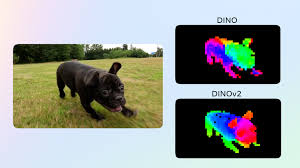
\includegraphics[width=0.7\textwidth]{figures/images.jpeg}
%     \caption{So sánh đặc trưng giữa DINO và DINOv2 (PCA features)}
%     \label{fig:dino_pca}
% \end{figure}

\subsection{Đóng góp chính (Contribution)}
Bài báo DINOv2 mang lại 3 đóng góp mang tính nền tảng cho tương lai của Computer Vision:
\begin{itemize}
    \item \textbf{Tiên phong cho "Thị giác thuần túy":} Đập tan định kiến cho rằng phải cần đến văn bản (text-supervision) mới tạo ra được mô hình nền tảng. DINOv2 chứng minh rằng hình ảnh tự bản thân nó chứa đủ lượng thông tin để mô hình học được các cấu trúc sâu sắc nhất.
    \item \textbf{Định hình lại cách xây dựng Dữ liệu lớn:} Đề xuất một quy trình chuẩn mực, tự động và mã nguồn mở để lọc dữ liệu hình ảnh khổng lồ (tạo ra tập LVD-142M), giải quyết bài toán thiếu hụt dữ liệu chất lượng cao trong kỷ nguyên SSL.
    \item \textbf{Dân chủ hóa AI thông qua Mã nguồn mở:} Meta đã công bố toàn bộ trọng số của các phiên bản DINOv2 (ViT-S, ViT-B, ViT-L, ViT-g). Ngay lập tức, DINOv2 đã trở thành "xương sống" (backbone) tiêu chuẩn được cộng đồng sử dụng rộng rãi để trích xuất đặc trưng cho vô số các nghiên cứu ứng dụng từ y tế, nông nghiệp đến xe tự lái.
\end{itemize}
